\section{LFSR as PRNG} \label{LFSR}

CC2538 User's Guide describes the PRNG design as: (Section 16.1 in CC2538 User's Guide)
\begin{quote}
The random-number generator is a 16-bit linear-feedback shift register (LFSR) with polynomial X 16 + X 15 +
X 2 + 1 (that is, CRC16). It uses different levels of unrolling depending on the operation it performs. The basic version (no unrolling) is shown in Figure 16-1 (\Cref{CRC16} in this paper).
\end{quote}

\begin{figure}[!t]
\centering
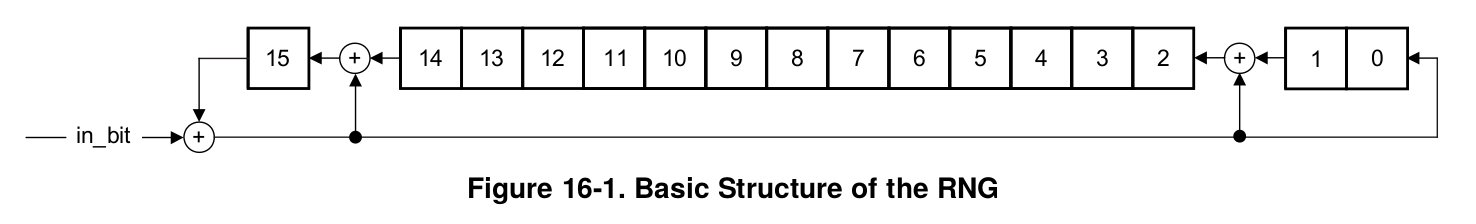
\includegraphics[width=2.5in]{fig/crc16.png}
\caption{CRC16 LFSR, from CC2538 User's Guide}
\label{CRC16}
\end{figure}

When used as a PRNG, the in\_bit in \Cref{CRC16} is constantly $0$. The Contiki driver calls the PRNG by: (Section 16.2.1in CC2538 User's Guide)
\begin{quote}
Another way to update the LFSR is to set the RCTRL bits in the SOC\_ADC\_ADCCON1 register to 01. This clocks the LFSR once (13x unrolling), and the RCTRL bits in the SOC\_ADC\_ADCCON1 register automatically clear when the operation completes.
\end{quote}

In another word, the LFSR is updated by performing 13 CRC16 operations in \Cref{CRC16} upon each RNG call. Since the CRC16 is deterministic and the register has only $16$ bits, the PRNG can be modelled as a Deterministic Finitee Automaton (DFA) which made its output easily predictable as we will explain later in this section.

Since there are only 16 bits in the LFSR, we can denote the universal set of its  possible values (or called states) $\mathbb{S}$ as:
\begin{equation} \label{PRNGState}
\mathbb{S} = \{ S_{i} | S_{i} \in \{2\}^{16}\}
\end{equation}
\Cref{PRNGState} implies that the LFSR can have no more than $|\mathbb{S}| = 2^{16} = 65536$ values.

We denote the LFSR update operation as:
\begin{equation}
F:\mathbb{S} \rightarrow \mathbb{S}
\end{equation}
where $F$ is $13$ times of CRC16 operation on the current state according to the manual.

Denote the 16 bits random seed sampled by the radio noise as $S^*$. The PRNG output can be formalised as:
\begin{equation}
	\begin{aligned}
	S_{0} &= S^* \\
	S_{i+1} &= F(S_{i})
	\end{aligned}
\end{equation}

Since ${S}$ is finite and $F$ is deterministic, the random number sequence will eventually results into a cyclic sequence. The maximum non-repetitive PRNG output sequence $R$ can be represented as:
\begin{equation} \label{R*}
R_{S^*}= (F^0(S^{*}), F^{1}(S^{*}), ..., F^{n-2}(S^{*}, F^{n-1}(S^{*}))
\end{equation}
where $S^{*} = F^{0}(S^{*}) = F^{n}(S^{*})$. Each call to the PRNG effectively returns the first element in the sequence and updates it by one cyclically left rotation. Since the sequence is non-repetitive, we have $n \leq |\mathbb{S}|$. In another word, the cycle of PRNG output can be no longer than $65536$ calls.

If a re-sampled seed $S^{*'}$ is inside $R_{S^*}$, i.e. $S^{*'} = F^{k}(S^*)$ where $k \in \mathbb{Z}_n$, then its corresponding maximum non-repetitive PRNG output sequence will be:
\begin{equation}\label{R*'}
	\begin{aligned}
	R_{S^{*'}} = &( F^{k}(S^*), F^{k+1}(S^{*}), ..., F^{n-1}(S^*), F^{0}(S^*), ...,\\
	&F^{k-2}(S^{*}), F^{k-1}(S^{*}))
	\end{aligned}
\end{equation}

Comparing \Cref{R*} to \Cref{R*'}, we can see that $R^*$ is actually $R^{*'}$ left cyclically rotated by $(n-k)$ times. This is equivalent to say that the PRNG sequence generated by $R^{*'}$ is identical to $R^*$ with $(n-k)$ preceding calls.

 As a result, assume consecutive calls to the PRNG seeded by $S^*$ generated a random number sequence:
\begin{equation*}
(S_i, S_{i+1}, ..., S_{j})
\end{equation*}
Then the same sequence can also be found during consecutive calls to a PRNG seeded by seed $S^{*'}$. This directly leads to the complete break of DTLS as we will explain in \Cref{BreakDTLS}.

This property also indicates that for a seed not inside $R_{S^*}$, its random number sequence will have no overlapping elements to $R_{S^*}$. By enumerating the 16 bit space of $\mathbb{S}$ (source code available at \cite{prngtest}), we found that there exists only four non-overlapping sequences that can be generated by the PRNG of CC2538:
\begin{itemize}
	\item $R_{0x0001}$ with $n = 32767$.
	\item $R_{0x0003}$ with $n = 32767$.
	\item $R_{0x0000}$ with $n = 1$.
	\item $R_{0x8003}$ with $n = 1$.
\end{itemize}
where $R_{0x0000}$ and $R_{0x8003}$ are excluded by the manual\cite{CC2538Manual}. 

\section{Breaking DTLS} \label{BreakDTLS}
tinydtls\cite{tinydtls} is a DTLS implementation on Contiki. For the currently available version 0.8.2\cite{tinydtls082},  two cipher suites are supported, namely Pre Shared Key (PSK) and ECDHE\_ECDSA\cite{rfc4492}. The only curve supported by the implementation is secp256r1\cite{secp256r1}. In this paper we only discuss ECDHE\_ECDSA.

%As explained in \Cref{LFSR}, the CC2538 PRNG output is a predictable stream of cycle less than $2^{16}$ calls; therefore the possible key selection can be easily enumerated and leads to a complete break of cryptographic systems relies on its randomness.    

tinydtls does not implement its own RNG; instead it invokes the Contiki RNG API (random\_rand()) in a loop to generate arbitrary length of random number (source code in tinydlts/dtls\_prng.h). When such RNG is used to generate an ECC key, the security notion is immediately broken as the random number is actually predictable as described in \Cref{LFSR}.
\begin{figure}
	\begin{algorithmic}[1]
	\scriptsize
	\REQUIRE Domain Parameter $T = (p, a, b, G, n, h)$ as specified by \cite{secp256r1}.
	\STATE Randomly select $d \in [1, n-1]$.
	\STATE Compute $Q = dG$.
	\RETURN $(Q,d)$, where $Q$ is the public key and $d$ the secret key.
	\end{algorithmic}
	\caption{ECC Key Generation}
	\label{KeyGen}
\end{figure}

 \Cref{KeyGen} describes the ECC Key Generation. The RNG is involved in the selection of $d$. Since $T$ is public, an adversary can pre-compute the all possible public keys by enumerating all secret keys beginning in each position of $R_{0x0001}$ and $R_{0x0003}$. Upon observing a public key, the adversary can immediately look up its corresponding secret key in the pre-computed look up table. Since the look up table has only $65534$ entries, the pre-computation took less than 5 minutes on a laptop powered by i7-2620M. 
 
Practically, the attack can be applied to two scenarios during a DTLS handshake:
\begin{itemize}
	\item \paragraph{\textbf{ECDSA}}
	ECDSA is an authentication scheme that allows a party to authenticate a message. In DTLS, it is used to sign the server parameters (details in \cite{rfc3279}) during the handshake to provide server side authenticity. \Cref{ECDSA} briefly describes the signing scheme of ECDSA. The adversary observing $(m,r,s)$ can revert $k$ by searching $r$ in the look up table. He can then recover the server secret key $d$ by computing:
	\begin{equation}
		\begin{aligned}
		e &= SHA-1(m) \\
		d &= r^{-1}(sk - e) \mod n
		\end{aligned}
	\end{equation}
	
	\begin{figure}
		\begin{algorithmic}[1]
		\scriptsize
		\REQUIRE Domain Parameter $T = (p, a, b, G, n, h)$, server key pair $(Q,d)$ and a message to be signed $m$.
		\STATE Randomly select $k \in [1, n-1]]$.
		\STATE Compute $kG = (x_1, y_1)$ and let $r = x_1 \mod n$.
		\STATE Compute $e = SHA-1(m)$.
		\STATE Compute $s = k^{-1}(e + dr) \mod n$.
		\RETURN $(m,r,s)$ as the message-signature pair.
		\end{algorithmic}
		\caption{ECDSA Signing}
		\label{ECDSA}
	\end{figure}
	
\item \paragraph{\textbf{ECDHE}}
	ECDHE is a key exchange protocol that allows two party to derive a shared secret. In DTLS, ECDHE is performed at the end of DTLS handshake to derive a shared symmetric key that is used for encrypting data packets. \Cref{ECDHE} provides a brief description of ECDHE. The adversary can recover $r_A$ and $r_B$ by observing $Q_A$ and $Q_B$ that is being sent in the packets; hence computes $K$ to derive the symmetric key.
	\begin{figure}
		\begin{algorithmic}[1]
		\scriptsize
		\REQUIRE Domain Parameter $T = (p, a, b, G, n, h)$. Party $A$'s key pair $(Q_A, d_A)$ and party $B$'s key pair $(Q_B, d_B)$. 
		\STATE $A$ randomly picks $r_A \in [0, n-1]$. 
		\STATE $B$ randomly picks $r_B \in [0, n-1]$.
		\STATE $A$ computes $Q_A = {r_A}G$ and sends $Q_A$ to $B$.
		\STATE $B$ computes $Q_B = {r_B}G$ and sends $Q_B$ to $A$.
		\STATE Both $A$ and $B$ computes $Q_{AB} = {r_A}{r_B}G = {r_A}{Q_B} = {r_B}{Q_A}$.
		\RETURN Both $A$ and $B$ returns $K = Hash(Q_{AB})$ as the shared secret.
		\end{algorithmic}
		\caption{ECDHE}
		\label{ECDHE}
	\end{figure}
\end{itemize}

We have tested the attacks by sniffing two CC2538 nodes performing handshake using the example code provided by tinydtls. The secret keys have been successfully recovered using the look up table we generated in \cite{prngtest}.

\section{Reflection on PRNG design}\label{PRNGReflection}
%Stdlib implementation
Investigating RNG implementations in other platforms supported by Contiki, we realised that most of them does not have a dedicated RNG implementation and by default wraps rand() in stdlib as the RNG. We then followed to some of the open sourced stdlib implementations. For the majority of the libraries, i.e. stdlib for ARM\cite{ARMrand}, AVR\cite{AVRrand} and MSP430\cite{MSP430rand}, the rand() implementation can be abstracted as \Cref{rand}. The type of variable \textit{seed}  may vary on different platforms. The \textit{do\_rand()} function outputs a congruent of linear transformation of \textit{seed} and updates it by the output.
 
\begin{figure}
\lstinputlisting[breaklines=true,basicstyle=\scriptsize]{src/rand.c}
\caption{rand() implementations in stdlib}
\label{rand}
\end{figure}

It is clear that such design would also yield into a predictable random number stream with cycle no longer than the range of \textit{seed}, as the same \textit{seed} will return the same output. On the above platforms, the cycles are no longer than $2^{32}$, $2^{16}$ and $2^{16}$ calls respectively.

%Improvements (NIST 800-90A)
As an improvement, we suggest to use more sophisticated PRNG implementation for cryptographic applications. \cite{NISTPRNG} has recommended several PRNG constructions based on approved hash functions and block ciphers. Specifically for CC2538, SHA-256 and AES have hardware coprocessor support and hence can be considered candidates for implementing cryptographically secure PRNG according to \cite{NISTPRNG}.

